\newpage
\section*{25~Jahre FOSSGIS~e.V. -- Willkommen zur FOSSGIS-Konferenz 2025 in Münster!}\label{welcome}

\begin{flushright}
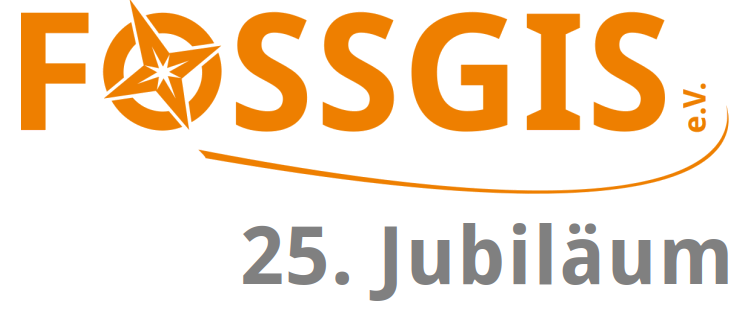
\includegraphics[width=1.0\textwidth]{Logo_Verein_25.png}
\end{flushright}

\noindent
Im Jahr 2025 wird der FOSSGIS e.V. 25 Jahre alt. Gegründet wurde der Verein als
GRASS Anwendervereinung (GAV e.V.) am 15.04.2000 in Hannover. Über die Zeit
kamen immer mehr Software-Projekte hinzu, weshalb der Verein im Jahr 2008 in
FOSSGIS e.V. umbenannt wurde. {\bfseries  FOSSGIS} steht für {\bfseries f}reie
{\bfseries O}pen"={\bfseries S}ource"={\bfseries S}oftware für
{\bfseries G}eo\-{\bfseries i}nformations\-{\bfseries s}ysteme.
Neben dem Thema \glqq Open-Source-Software\grqq wurde auch das
Thema der offenen Geodaten immer wichtiger. Seit 2017 ist der FOSSGIS~e.V.
auch der offizielle Vertreter des OpenStreetMap-Projektes in Deutschland.

\noindent
Kern unserer Arbeit ist die jährliche FOSSGIS-Konferenz, die Entwickler und
Nutzende zusammenbringt. Wir sind aber auch über die Konferenzen hinaus aktiv,
gehen zu Veranstaltungen, beantworten Fragen in Online-Foren oder betreuen
die digitale Infrastruktur hinter den Projekten.

\pagebreak
\noindent
Die Nachfrage nach Informationen und Vernetzung steigt stetig an. Dies zeigt sich
an den Teilnehmerzahlen der Konferenzen, wie auch an der Zahl der E-Mails und
Telefonanrufe, die uns täglich erreichen. Daher hat der Verein seit fünf Jahren
eine professionelle Koordinierungsstelle, die die ehrenamtliche Arbeit
unterstützt und als Schnittstelle nach Außen dient. Ende 2023 wurde die
Koordinierungsstelle speziell für den OSM-Bereich erweitert.

\noindent
Nach wie vor wird die meiste Arbeit im Verein von Ehrenamtlichen getragen.
Dazu braucht es Menschen, die mitmachen und sich engagieren, Ideen einbringen
und unsere Zukunft mitgestalten wollen. Vielleicht kommen Sie mal am
FOSSGIS-Stand vorbei und reden Sie mit uns! Wir freuen uns auf Ihre Fragen und
Ideen und vielleicht haben Sie ja auch Lust mitzumachen!

\noindent
Die {\bfseries FOSSGIS-Konferenz 2025} wird vom gemeinnützigen FOSSGIS e.V. und der
OpenStreetMap-Community in Kooperation mit dem Institut für Geoinformatik der
Universität Münster veranstaltet. 
Die FOSSGIS-Konferenz ist eine Communityveranstaltung und wird vorwiegend
ehrenamtlich organisiert.
Ziel der Konferenz ist die Verbreitung von freier, quelloffener Software für
Geoinformationssysteme. In den nächsten vier Tagen haben Sie die Gelegenheit,
sich mit Entwickler:innen und anderen Anwender:innen auszutauschen und
neueste Informationen zu Anwendungen und Arbeitsmöglichkeiten zu erhalten.

\pagebreak
\noindent
Konferenzbeiträge zum Vereinsjubiläum:
\begin{description}
\item{\bfseries Mittwoch, 10:30 im Eröffnungsblock:} 25~Jahre FOSSGIS~e.V. - in der Zeitreise durch das Vereinsleben werden verschiedene Mitglieder und Aktive aus dem FOSSGIS~e.V. Aktivitäten, Highlights, Erinnerungen, Erfahrungen, Geschichten aus der Vereinsarbeit teilen.
\item{\bfseries Mittwoch 17:40 - 18:40 \HSeins:} Podiumsgespräch zu 25~Jahre FOSSGIS e.V. - was haben wir geschafft und wo wollen wir hin.
%\item{\bfseries Donnerstag 19:00 \BoFeins:} Mitgliederversammlung des FOSSGIS~e.V. - Gäste sind willkommen.
\item{\bfseries Freitag 15:15 \HSeins:} Ein Blick in die Koordinierungsstelle des FOSSGIS~e.V.
\end{description}

\section*{Exkursionen {\normalfont\em (Anmeldung erforderlich)}}\label{exkursionen}
\noindent
{\large \bfseries Führung durch die Kartensammlung des Landesarchiv NRW}\\
Es wird durch das Magazin des Landesarchiv NRW Abteilung Westfalen geführt. Der Schwerpunkt liegt auf der Kartensammlung und umfasst Karten und Archivgut vom 16. Jahrhundert bis in die Gegenwart. {\bfseries Freitag, 28.03.2025, 17:00} Treffpunkt: Landesarchiv NRW Abteilung Westfalen, Bohlweg 2.
\bigskip

\noindent
{\large \bfseries Archäologisch historischer Stadtrundgang}\\
Vom Domplatz geht es zur Überwasserkirche (dort eine Ausgrabung wegen Fernwärmebau, besonders interessantes Siedlungsgebiet) und weiter zur Jüdefelderstraße. Über den Buddenturm und Zwinger zum Mauritztor von dort aus über den alten Fischmarkt zum Prinzipalmarkt. Auf dem Rundgang werden abgeschlossene und aktuelle Ausgrabungsstellen sowie archäologisches Arbeiten (Vermessungsdaten, Planerstellung, Datenablage etc.) im städtischen Raum vorgestellt. {\bfseries Samstag, 29.03.2025, 14:00~Uhr }, Treffpunkt: S-Bahn Haltestelle Stadthausbrücke, Bahnsteig, Aufgang zur Michaeliskirche.
\bigskip

\section*{Abendveranstaltung am Mittwoch}\label{schwaetzli}
Am ersten Abend der FOSSGIS-Konferenz findet die Abendveranstaltung in der Mensa am Aasee (Bismarckallee~11, 48151~Münster) von {\bfseries 19:00 bis 22:00 Uhr} statt. Eine Anmeldung ist erforderlich.

\section*{Rahmenprogramm am Donnerstag}
\subsection*{Gruppenfoto}
Auch in diesem Jahr wollen wir uns das Gruppenfoto nicht entgehen lassen und laden Sie am {\bfseries Donnerstag} in der {\bfseries Nachmittagspause} zum Gruppenfoto ein am Haupteingang des Schloss Münster.

\subsection*{Mitgliederversammlung des FOSSGIS e.V.}
Am {\bfseries Donnerstag} sind alle Mitglieder und Gäste ab {\bfseries 19.00 Uhr} herzlich zur Mitgliederversammlung des FOSSGIS e.V. eingeladen zum Diskutieren, Kennenlernen und Abstimmen. Ab 18:30 Uhr
gibt es Getränke und Pizza für alle. Der Verein freut sich über zahlreiches Erscheinen.

\section*{Rahmenprogramm am Freitag}

\subsection*{Sektempfang am FOSSGIS-Stand}
Alle Mitglieder des FOSSGIS-Vereins, Freunde und Interessierte sind am {\bfseries Freitag} ab {\bfseries 16.30 Uhr} herzlich zum Sektempfang zum Ausklang der FOSSGIS 2024 am FOSSGIS-Vereins-Stand eingeladen.

\subsection*{OSM-Event am Freitagabend}
Für alle, die am {\bfseries Freitagabend} noch in der Stadt sind und/oder am OSM-Event teilnehmen möchten, wird ein Treffpunkt bekanntgegeben.

\pagebreak
\section*{OSM-Samstag}
Am Samstag, den 29.~März findet von 9.00 bis 17.30~Uhr die OSM-Unkonferenz statt.
Interessierte sind eingeladen sich zu beteiligen oder daran teilzunehmen.
Die Themensammlung erfolgt im OSM-Wiki. Die Veranstaltung ist kostenfrei.
Um Anmeldung über das FOSSGIS-Konferenz-Anmeldesystem wird gebeten.

\subsection*{Community-Sprint}
Beim Community-Sprint wird gemeinsam an OpenSource Projekten gearbeitet.
Die Veranstaltung startet um 9~Uhr mit einem kurzen Vortrag, der für Einsteiger:innen
und Interessierte erklärt wie OpenSource funktioniert und wie man beitragen kann.
Im Anschluss wird gemeinsam oder individuell an Projekten gearbeitet.
Um Anmeldung über das FOSSGIS-Konferenz-Anmeldesystem wird gebeten.
